\documentclass[serif,xcolor=pdftex,dvipsnames,table,hyperref={bookmarks=false,breaklinks}]{beamer}

%%%%%%%%%%%%%%%%
% Change the macros below to configure the title slides
% for your course.
\newcommand{\coursename}{COMPSCI 589}
\newcommand{\instructor}{Benjamin M. Marlin}
\newcommand{\university}{University of Massachusetts Amherst}
\newcommand{\department}{College of Information and Computer Sciences}
%%%%%%%%%%%%%%%%


\newcommand{\settitlecard}[2]{
  \title[\coursename  Lecture #1] 
    {\coursename \\ Lecture #1: #2}
     \author[\instructor]{\instructor}
     \institute[\university]{
     \department\\
     \university
   }
\date{}
}

\newcommand{\maketitlepage}{
  \begin{frame}
  \titlepage
  \center{
    %If you use the slides unmodified, retain the attribution below
    \tiny{Slides by Benjamin M. Marlin (marlin@cs.umass.edu). \\
    \vspace{-1em}Created with support from National Science Foundation Award\# IIS-1350522. 
    %If you modify the slides, please retain the alternate attribution below
    %\tiny{Based on slides by Benjamin M. Marlin (marlin@cs.umass.edu). \\    
    %\vspace{-1em}Created with support from National Science Foundation Award\# IIS-1350522. 
    }                                              
  }  
  \end{frame}
}

\AtBeginSection[]
{
  \begin{frame}<beamer>{Outline}
    \tableofcontents[currentsection,subsectionstyle=hide]
  \end{frame}
}


\newcommand{\cut}[1]{}

\newcommand{\iconbox}[4]{
  \only<#1-#2>{
    \begin{columns}[T]
      \column{0.5in}
           \includegraphics[width=0.5in]{#3}
       \column{3.7in}
            #4
    \end{columns}
    \medskip
    \medskip
    \medskip
  }
}

\mode<presentation>{
  \usepackage{../beamertheme589theme}
  \setbeamercovered{invisible}
}

\mode<handout>{
  \usepackage{../beamertheme589theme}
  \setbeamercovered{transparent}
}


\usepackage[english]{babel}
\usepackage[latin1]{inputenc}
\usepackage{times}
\usepackage[T1]{fontenc}
\usepackage{amsmath}
\usepackage{amssymb}
\usepackage[noend]{algorithmic}
\usepackage{algorithm}
\usepackage{listings}

\renewcommand\mathfamilydefault{\rmdefault}

\newcommand{\setA}{\mathcal{A}}
\newcommand{\setB}{\mathcal{B}}
\newcommand{\setS}{\mathcal{S}}
\newcommand{\setV}{\mathcal{V}}
\DeclareMathOperator*{\union}{\bigcup}
\DeclareMathOperator*{\intersection}{\bigcap}
\DeclareMathOperator*{\Val}{Val}
\newcommand{\mbf}[1]{{\mathbf{#1}}}
\DeclareMathOperator*{\argmax}{arg\,max}
\DeclareMathOperator*{\argmin}{arg\,min}
\DeclareMathOperator*{\sign}{sign}
\newcommand{\deriv}[2]{\frac{\partial{#1}}{\partial{#2}}}


\settitlecard{18}{Linear Dimensionality Reduction and SVD}

\begin{document}

\maketitlepage

\section{Dimensionality Reduction}
\subsection{Foo}

\begin{frame}[t]{Machine Learning Tasks}
 \centering
 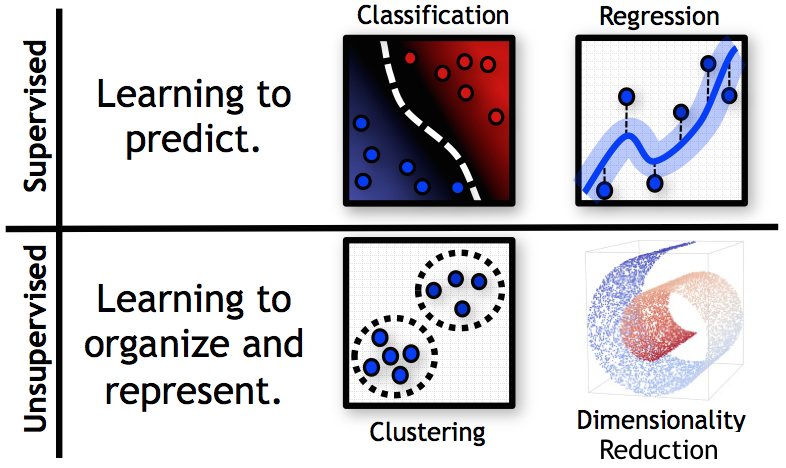
\includegraphics[width=4in]{../Figures/learning_problems.png}
\end{frame}


\begin{frame}[t]{The Dimensionality Reduction Task}

\begin{block}{Definition: The Dimensionality Reduction Task}
Given a collection of feature vectors $\mbf{x}_i\in\mathbb{R}^D$, map the 
feature vectors into a lower dimensional space $\mbf{z}_i\in\mathbb{R}^K$ where 
$K<D$ while preserving certain properties of the data.
\end{block}

\pause
\center
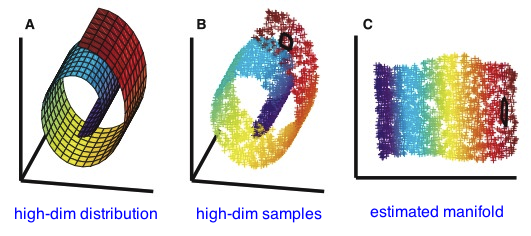
\includegraphics[width=4in]{../Figures/manifold_unrolling.png}
\end{frame}

\begin{frame}[t]{Example: Representing Time Series}
\center
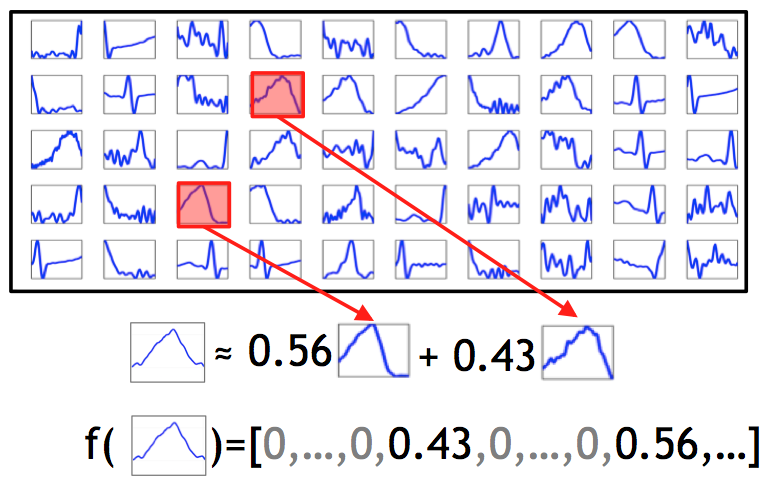
\includegraphics[width=4in]{../Figures/spase_coding_time_series.png}
\end{frame}

\begin{frame}[t]{Example: Learning Face Parts}
\center
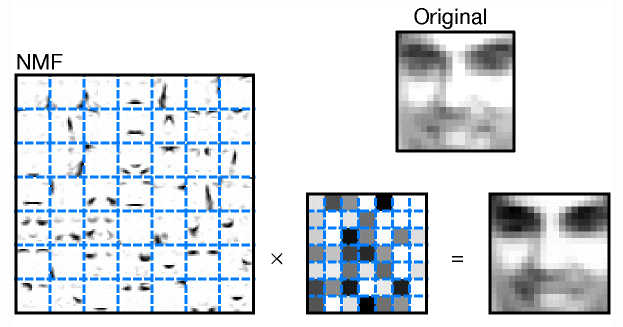
\includegraphics[width=4.5in]{../Figures/nmf.png}
\end{frame}

\begin{frame}[t]{Example: Representing Natural Image Patches}
\center
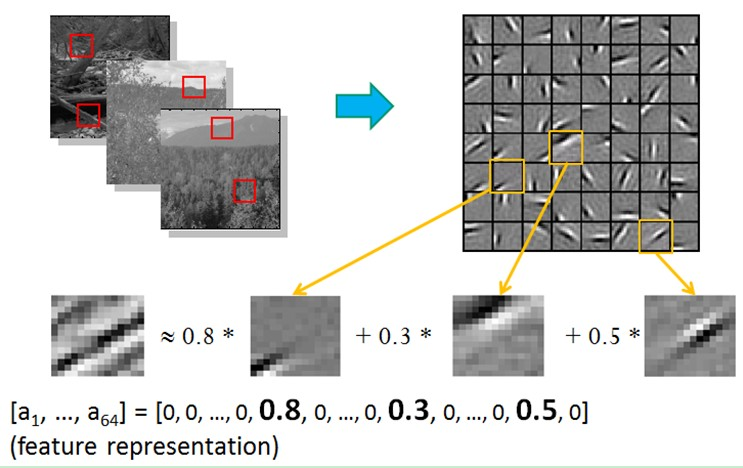
\includegraphics[width=4.5in]{../Figures/sparse_coding_images.jpg}
\end{frame}

\begin{frame}[t]{Example: Image Embedding}
\center
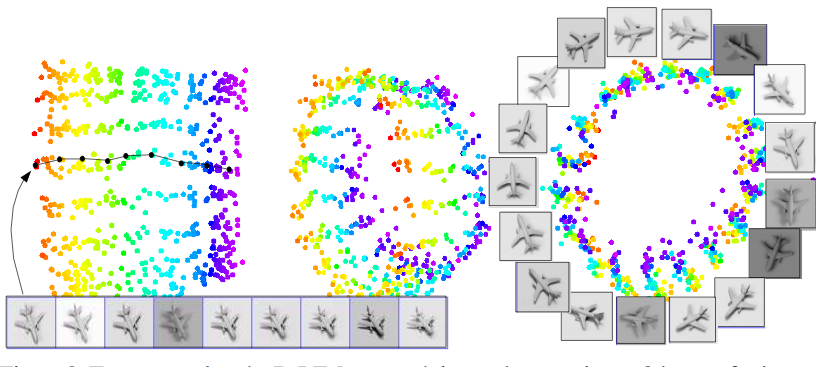
\includegraphics[width=4.5in]{../Figures/image_embedding.png}
\end{frame}

\begin{frame}[t]{Applications}
 
\begin{itemize}
\item Can be used as a pre-processing step to enable more accurate
classification and regression on manifold data.

\pause \item Very low dimensional embeddings (ie: K=2,3) can be used to
visualize complex manifold-structured data as in the previous example.

\pause \item Can be used to de-noise data by projecting to lower-dimensional
space and then projecting back to the feature space.

\end{itemize} 
\end{frame}

\begin{frame}[t]{Dimensionality Reduction vs Feature Selection}
 
\begin{itemize}
\item The goal of feature selection is to remove features that are not 
informative with respect to the class label. This obviously reduces the 
dimensionality of the feature space.

\pause\item Dimensionality reduction can be used to compress the feature space
for manifold structured data even when there is information in each of the 
feature dimensions so that none can be discarded.

\pause\item Another important property of dimensionality reduction is that it is 
unsupervised. It will attempt to preserve structure in the data that could be
useful for a range of supervised problems, not a specific problem. 

\pause\item Unlike feature selection, which is a supervised task, 
dimensionality reduction can sometimes compress out structure useful to a 
particular supervised task thereby increasing error.

\end{itemize} 
\end{frame}


\section{Linear Dimensionality Reduction}
\subsection{Foo}

\begin{frame}[t]{Linear Dimensionality Reduction}
 
\begin{itemize}
\item The simplest dimensionality reduction methods assume that the observed 
high dimensional data vectors $\mbf{x}_i\in \mathbb{R}^D$ lie on a 
K-dimensional linear manifold within $\mathbb{R}^D$. 

\center
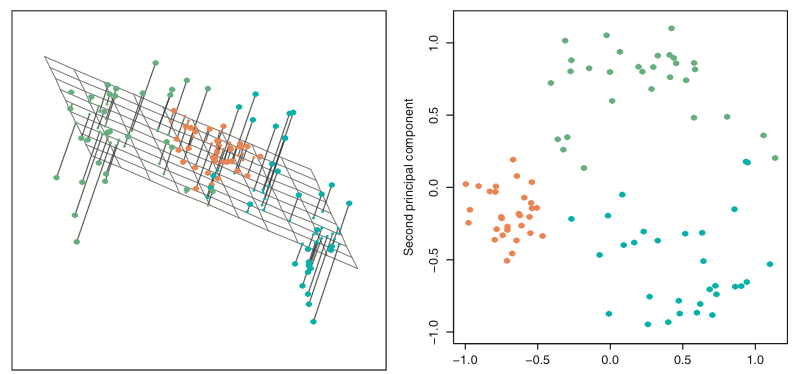
\includegraphics[width=4in]{../Figures/linear_subspace.png}


\end{itemize} 
\end{frame}

\begin{frame}[t]{Linear Dimensionality Reduction}
 
\begin{itemize}
\item Mathematically, the linear sub-space assumption can be written as follows:

{\Large
$$\mbf{x}_{id} = \sum_{k=1}^K z_{ik} b_{kd}$$
}

where $\mbf{b}_k=[b_{k1},...,b_{kD}]$ for $k=1,...,K$ are a 
set of basis vectors describing a $K$-dimensional linear sub-space of 
$\mathcal{R}^{D}$ and $z_{ki}$ are a set of real-valued weights on those basis 
vectors.


\end{itemize} 
\end{frame}


\begin{frame}[t]{Connection to Linear Regression}
 
\begin{itemize}
\item This expression is exactly linear regression where $x_{id}$ is 
the target, $z_{ik}$ are the weights, and $\mbf{b}_{kd}$ for each $k$ are the 
features. 

{\Large
$$\mbf{x}_{id} = \sum_{k=1}^K z_{ik} b_{kd}$$
}

\pause\item This observation is also true if we swap the roles of the weights 
and the features.

\pause\item However, unlike the linear regression case, we only know what 
corresponds to the targets. We must learn both the features and the weights. 

\end{itemize} 
\end{frame}

\begin{frame}[t]{Matrix Form}
 
\begin{itemize}
\item If we let $\mbf{X}$ be the data matrix $\mbf{X}_{id}= x_{id}$,
$\mbf{Z}$ be a matrix where $\mbf{Z}_{ik}=z_{ik}$, and $\mbf{B}$ be a matrix 
where $\mbf{B}_{kd}=b_{kd}$, we can express $\mbf{X}$ as follows:

{\Large
$$\mbf{X} = \mbf{Z}\times \mbf{B}$$
}

\pause\item $\mbf{Z}\in \mathbb{R}^{N\times K}$ is often referred to as the 
factor loading matrix while $\mbf{B}\in \mathbb{R}^{K\times D}$ are referred to 
as the latent factors by analogy to regression.

\end{itemize} 
\end{frame}

\begin{frame}[t]{Observation Noise}
 
\begin{itemize}
\item Most real world data will be subject to noise. If we assume that 
$\epsilon \in \mathbb{R}^{N\times D}$ is a matrix of noise values from some
probability distribution, we have:

{\Large
$$\mbf{X} = \mbf{Z}\times \mbf{B} + \epsilon$$
}

\end{itemize} 
\end{frame}

\begin{frame}[t]{Learning}
 
\begin{itemize}
\item The learning problem for linear dimensionality reduction is to estimate
values for both $\mbf{Z}$ and $\mbf{B}$ given only the noisy observations 
$\mbf{X}$.

\pause\item One possible learning criteria is to minimize the sum of squared 
errors when reconstructing $\mbf{X}$ from $\mbf{Z}$ and $\mbf{B}$. This leads 
to:

{\Large
$$\argmin_{\mbf{Z},\mbf{B}} ||\mbf{X} - \mbf{Z}\mbf{B} ||_F$$
}

where $||\mbf{A}||_F$ is the Frobenius norm of matrix  $\mbf{A}$ (the sum of 
the squares of all matrix entries). 

\end{itemize} 
\end{frame}

\begin{frame}[t]{Learning Algorithm}
 
\begin{itemize}
\item Not surprisingly, we can obtain a solution to this learning problem by
leveraging the OLS solution to linear regression. The algorithm is often 
referred to as Alternating Least Squares or ALS. 

\pause\item Starting from a random initialization, ALS iterates between 
assuming $\mbf{Z}$ are known features and optimizing $\mbf{B}$ 
as the unknown weights, and assuming that $\mbf{B}$ are the known features and 
optimizing $\mbf{Z}$ as the unknown weights:


{\Large
$$\mbf{B} \leftarrow (\mbf{Z}^T\mbf{Z})^{-1}\mbf{Z}^TX$$
$$\mbf{Z}^T \leftarrow (\mbf{B}\mbf{B}^T)^{-1}\mbf{B}X^T$$
}

\end{itemize} 
\end{frame}

\begin{frame}[t]{Lack of Uniqueness of Optimal Parameters}
 
\begin{itemize}
\item Suppose we run the ALS algorithm to convergence and obtain estimates
for $\mbf{Z}_*$ and $\mbf{B}_*$ such that:

$$c = ||\mbf{X} - \mbf{Z}_*\mbf{B}_*||_F$$

\pause\item Note that if we let $\mbf{R} \in \mathbb{R}^{K\times K}$ be an 
arbitrary $K\times K$ invertible matrix, then we obtain exactly the same value 
$c$ of the objective function for the alternate parameters 
$\tilde{\mbf{Z}}=\mbf{Z}_*\mbf{R}$ and $\tilde{\mbf{B}} = 
\mbf{R}^{-1}\mbf{B}_*$:

\begin{align*}
c &= ||\mbf{X} - \mbf{Z}_*(I)\mbf{B}_*||_F\\
 &= ||\mbf{X} - \mbf{Z}(\mbf{R}\mbf{R}^{-1})\mbf{B} ||_F\\
 &= ||\mbf{X} - \tilde{\mbf{Z}}\tilde{\mbf{B}} ||_F
\end{align*}

\end{itemize} 
\end{frame}

\begin{frame}[t]{Singular Value Decomposition}
 
\begin{itemize}
\item Interestingly, this optimization problem has a continuous subspace of 
optimal solutions that all obtain the same global minimum value of the 
objective function. 

\pause\item Each optimal solution is simply a different representation the same
linear subspace.

\pause\item We can pick a unique representation for the subspace by 
specifying additional criteria. Classical Rank-K Singular Value Decomposition 
(K-SVD) corresponds to the following restriction:

$$\argmin_{\mbf{U},\mbf{S},\mbf{V}} ||\mbf{X} - \mbf{U}\mbf{S}\mbf{V}^T ||_F$$

where $S$ is a $K\times K$ diagonal matrix with positive elements,  
$\mbf{U}$ is an $N\times K$ matrix such that  $\mbf{U}^T\mbf{U}=I$, and $V$
is a $DxK$ matrix such that $\mbf{V}^T\mbf{V}=I$.

\end{itemize} 
\end{frame}

\begin{frame}[t]{Trade-Offs}
 
\begin{itemize}
\item Minimum Frobenius norm linear dimensionality reduction is nice because 
it will find the globally optimal linear sub-space, and SVD provides a 
unique representation for this sub-space.

\pause\item The basic ALS algorithm scales as $O(K^3 + D^3)$ per pair of 
iterations due to the matrix inverses, which is not suitable for high 
dimensions. The full SVD algorithm scales as $O(min(DN^2, ND^2))$, which also 
isn't scalable to large data. However, fast approximations exist for both 
problems.

\pause\item A significant limitation of linear dimensionality reduction is that
it can fail to achieve a useful compression of the data if the underlying 
manifold is not actually linear.

\pause\item As with clustering, the rank $K$ of the latent sub-space is a free 
parameter.

\end{itemize} 
\end{frame}




\end{document}
